\section{Details of Experiment}
\label{sec:appendix_experiment}

\subsection{Training Hyperparameters}

\begin{table}[t]
    \centering
    \caption{\bf Detailed experimental settings.}
    \vspace{-1em}
    \label{tbl:appendix_hyperparameters}
    
    % --- Subtable 1: Operator Learning ---
    \begin{subtable}[t]{\columnwidth}
        \centering
        \caption{\bf{Hyperparameters for Operator Learning.}}
        \label{subtbl:hyper_op_learning}
        \vspace{-0.15em}
        \resizebox{0.5\linewidth}{!}{
        \begin{tabular}{|l||c|}
            \hline
            \textbf{Hyperparameter} & \textbf{Value} \\
            \hline \hline
            Base Model & Qwen3-8B \\
            Global Batch Size & 256 \\
            Learning Rate & 1e-5 \\
            Epochs & 3 \\
            Max Sequence Length & 16,384 \\
            Warmup Ratio & 0.05 \\
            Precision & bfloat16 \\
            \hline
        \end{tabular}
        }
    \end{subtable}
    
    \vspace{0.30em}
    
    % --- Subtable 2: Cold Start SFT ---
    \begin{subtable}[t]{\columnwidth}
        \centering
        \caption{\bf{Hyperparameters for Tree-based Agentic Reasoning SFT.}}
        \label{subtbl:hyper_cold_start}
        \vspace{-0.15em}
        \resizebox{0.5\linewidth}{!}{
        \begin{tabular}{|l||c|}
            \hline
            \textbf{Hyperparameter} & \textbf{Value} \\
            \hline \hline
            Base Model & Stage 1 Ckp \\
            Global Batch Size & 256 \\
            Learning Rate & 6e-5 \\
            Epochs & 15 \\
            Max Sequence Length & 24,000 \\
            Warmup Ratio & 0.05 \\
            Precision & bfloat16 \\
            \hline
        \end{tabular}
        }
    \end{subtable}
    
    \vspace{0.30em}
    
    % --- Subtable 3: RL ---
    \begin{subtable}[t]{\columnwidth}
        \centering
        \caption{\bf{Hyperparameters for Multi-Turn RL.}}
        \label{subtbl:hyper_rl}
        \vspace{-0.15em}
        \resizebox{0.5\linewidth}{!}{
        \begin{tabular}{|l||c|}
            \hline
            \textbf{Hyperparameter} & \textbf{Value} \\
            \hline \hline
            Algorithm & GRPO \\
            Global Batch Size & 64 \\
            Learning Rate & 1e-6 \\
            Epochs & 1 \\
            Group Size ($G$) & 8 \\
            KL Coefficient ($\beta$) & 0.005 \\
            Temperature / Top-p & 0.6 / 0.95 \\
            Max Total Length & 28,000 \\ 
            Max Response Length & 2000 \\
            Max Exploration Turn & 5 \\
            Max Prompt Length & 12000 \\
            \hline
        \end{tabular}
        }
    \end{subtable}
    
\end{table}


In this section, we provide the detailed implementation details and hyper-parameters for the three training stages of \sys: Operator Syntax Learning, Reasoning Procedure Learning, and Multi-turn RL with Hybrid Reward. Table~\ref{tbl:appendix_hyperparameters} summarizes the specific hyperparameters for each stage.

\stitle{Stage 1: Operator Syntax Learning}
As defined in Section~\ref{subsec:cold_start}, the goal of this stage is to focus on the syntax and semantics of individual operators. 
We set the learning rate to 1e-5 with a cosine scheduler and a warmup ratio of 0.05. Since this stage mainly involves generating short operator sequences, we set the maximum sequence length to 16,384. We train the model for 3 epochs with a global batch size of 256.

\stitle{Stage 2: Reasoning Procedure Learning}
This stage corresponds to aligning the model with the ``Agentic Tree-based Reasoning'' mechanism in Section~\ref{subsec:cold_start}. We initialize the model using the checkpoint from Stage 1. The objective is to teach the model to perform global planning, exploration, and backtracking using the agentic reasoning tree.
To accommodate the large context of the agentic reasoning tree and multi-turn interaction history, we increase the maximum sequence length to 24,000. We use a learning rate of 6e-5 to effectively learn the complex reasoning patterns. The training runs for 15 epochs with a global batch size of 256.

\stitle{Stage 3: Multi-turn RL with Hybrid Reward}
In the final stage, we apply the ``Multi-turn RL with Hybrid Reward'' described in Section~\ref{subsec:rl_reward}. We utilize the Group Relative Policy Optimization (GRPO) algorithm to optimize the model's decision-making strategy.
During training, we sample $G=8$ trajectories for each prompt to estimate the baseline. We use a small learning rate of 1e-6 and set the KL divergence coefficient ($\beta$) to 0.005 to ensure training stability.
To handle long-horizon tasks, we set the maximum total length to 28,000 and the maximum prompt length to 12,000. We limit the maximum exploration turns to 5 and the response length for each step to 2,000 tokens.
% We set $\alpha, \beta, \gamma$ in the hybrid reward (Section~\ref{subsec:rl_reward}) to 

\subsection{Training Data}

Due to time and computational constraints, we utilized a curated subset of the synthesized data for training rather than the full dataset. 
For the initial stage, we constructed a dataset of 8,000 samples. These samples focus on basic operator usage to establish the model's fundamental understanding of the operator space. 
In the SFT stage, we employed the five open-source LLMs mentioned in Section~\ref{subsec:exp-setup} as teacher models to generate diverse reasoning trajectories. We initially distilled approximately 20,000 trajectories. To ensure high training quality, we filtered these trajectories based on the process reward function $R_{\text{llm}}$ score (retaining scores $> 0.8$) and the number of interaction turns. This process yielded a final dataset of 11,198 high-quality samples. 
For the reinforcement learning stage, we randomly sampled 4,000 instances from the Synth-Spider dataset. These samples serve as the environment for the model to explore and optimize its policy via the hybrid reward signal.

% \subsection{Statistics of Exp-\ref{exp:evaluate_on_various_diff} on Other LLMs}

% \begin{figure}[t]
    \centering
    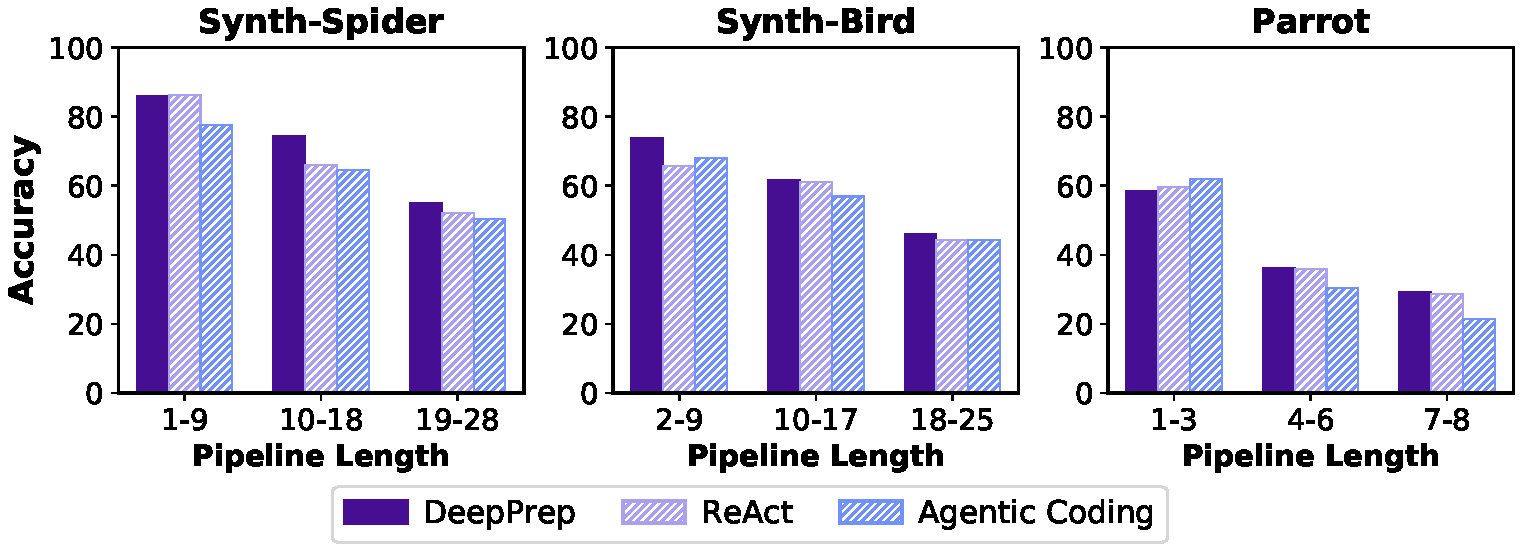
\includegraphics[width=0.99\columnwidth]{plots/plot/performance_compare_on_task_diff_gpt5.pdf}
    \vspace{-1em} 
    \caption{Performance Compare of different methods based on GPT-5 on cases with various difficulty.}
    \label{fig:performance_compare_on_task_diff_gpt5}
    \vspace{-1em}
\end{figure}
% \begin{figure}[t]
    \centering
    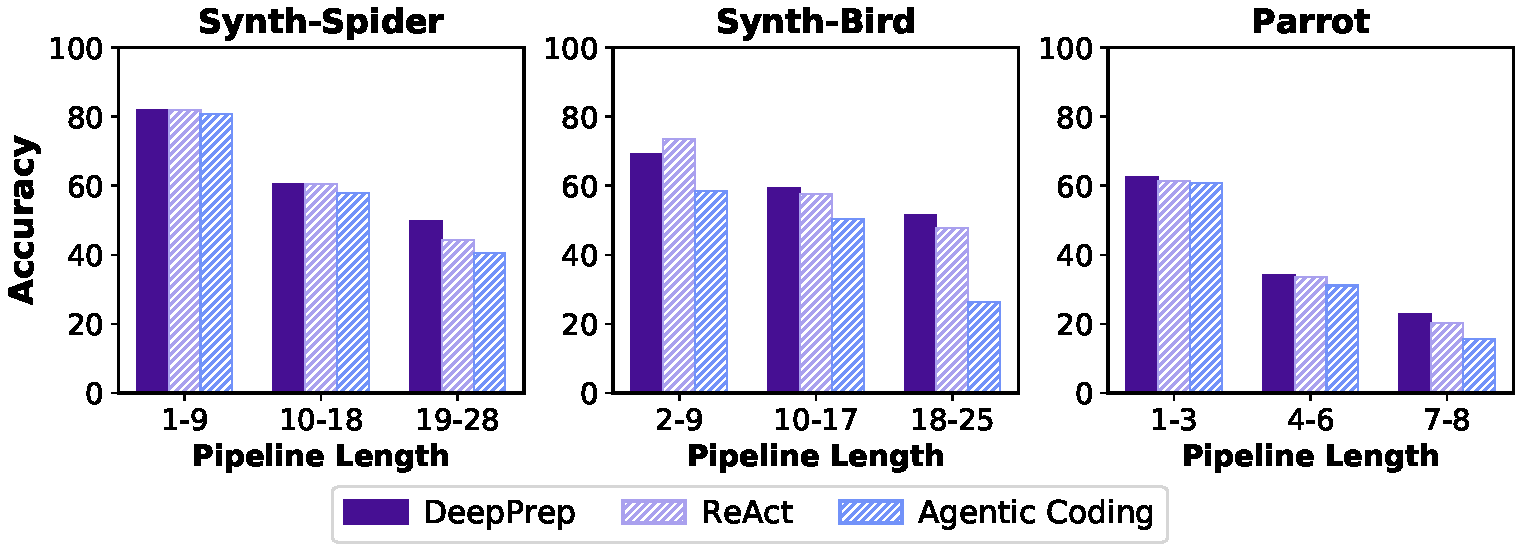
\includegraphics[width=1.01\columnwidth]{plots/plot/performance_compare_on_task_diff_r1.pdf}
    \vspace{-1em} 
    \caption{Performance Compare of different methods based on DeepSeek-R1 on cases with various difficulty.}
    \label{fig:performance_compare_on_task_diff_r1}
    \vspace{-1em}
\end{figure}
% \begin{figure}[t]
    \centering
    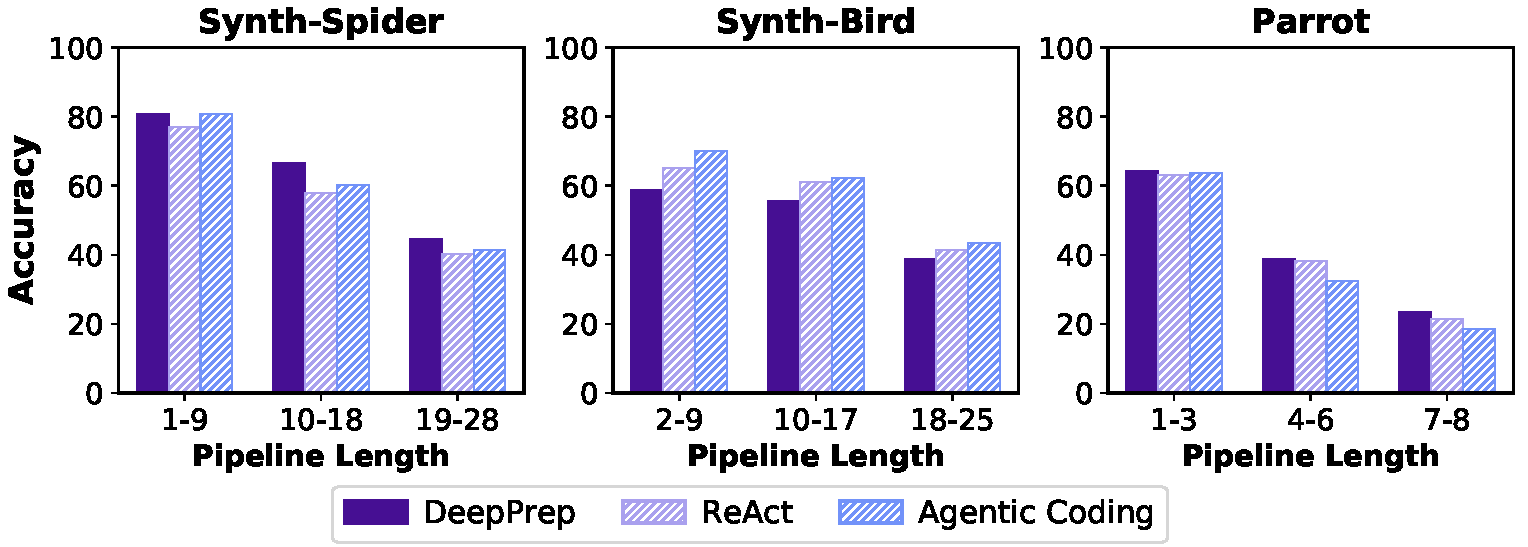
\includegraphics[width=0.99\columnwidth]{plots/plot/performance_compare_on_task_diff_doubao.pdf}
    \vspace{-1em} 
    \caption{Performance Compare of different methods based on DoubaoSeek-1.6 on cases with various difficulty.}
    \label{fig:performance_compare_on_task_diff_doubao}
    \vspace{-1em}
\end{figure}
% \begin{figure}[t]
    \centering
    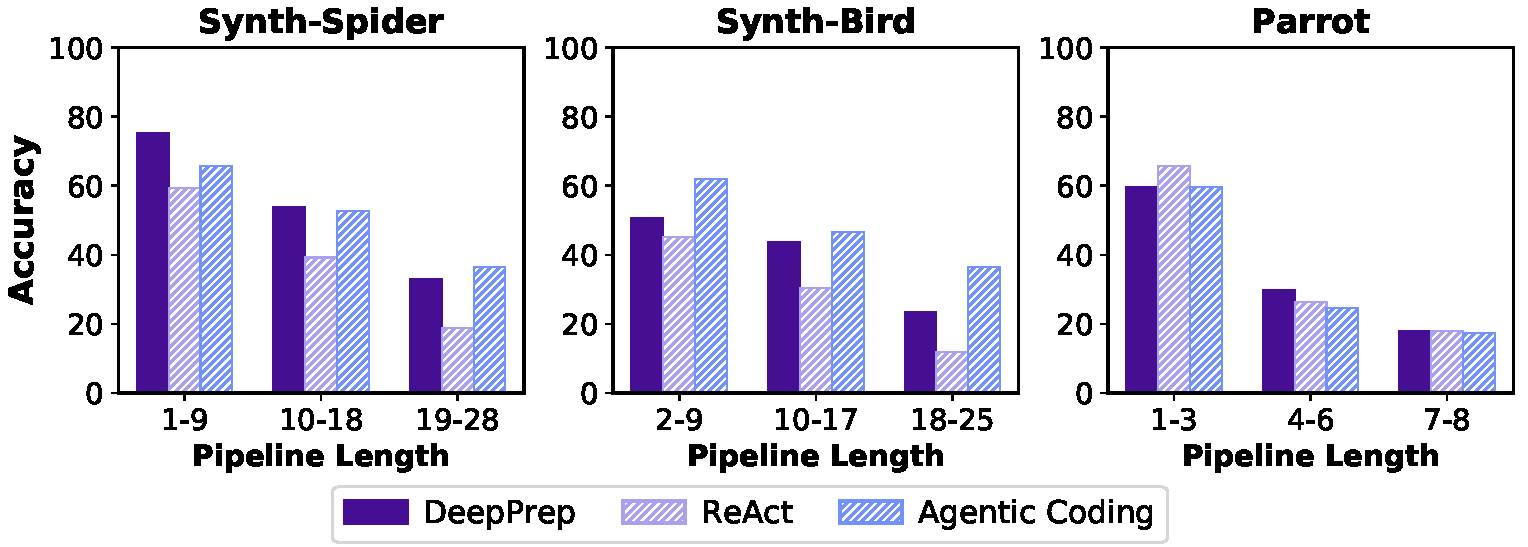
\includegraphics[width=0.99\columnwidth]{plots/plot/performance_compare_on_task_diff_v3.1.pdf}
    \vspace{-1em} 
    \caption{Performance Compare of different methods based on DeepSeek-V3.1 on cases with various difficulty.}
    \label{fig:performance_compare_on_task_diff_v3.1}
    \vspace{-1em}
\end{figure}

% In Section~\ref{sec:exp}, we demonstrated the robustness of \sysp on tasks of varying difficulty using the Claude-4 backbone. In this section, we also report the results of four additional LLMs with varying reasoning capabilities: GPT-5, DeepSeek-R1, DoubaoSeed-1.6 and DeepSeek-V3.1. The detailed comparisons are presented in Figure~\ref{fig:performance_compare_on_task_diff_gpt5}-\ref{fig:performance_compare_on_task_diff_v3.1}.

% As illustrated in the figures, consistent with the observations in Experiment~\ref{exp:evaluate_on_various_diff}, \sysp generally exhibits a widening performance gap over baselines as the task difficulty increases. 
% On \textit{Simple} subsets, linear reasoning methods like ReAct and CodeGen often achieve competitive results, as the operator pipelines are short and require less planning. 
% However, on \textit{Complex} subsets involving long-horizon dependencies, \sysp maintains a distinct advantage. This confirms that the tree-based exploration mechanism effectively mitigates error accumulation, which is the primary bottleneck for linear baselines in complex scenarios.

% Moreover, we observe a correlation between the reasoning capability of backbone models and the performance of \sysp.
% As shown in Figure~\ref{fig:performance_compare_on_task_diff_r1} and Figure~\ref{fig:performance_compare_on_task_diff_gpt5}, stronger backbones can fully leverage the global state tree to perform effective backtracking. For instance, with DeepSeek-R1 on the DP-Spider (Complex) subset, \sysp significantly outperforms the baselines. The strong instruction-following and reasoning abilities of these models allow them to navigate the search space efficiently.
% While for relatively weaker backbones (Figure~\ref{fig:performance_compare_on_task_diff_doubao} and Figure~\ref{fig:performance_compare_on_task_diff_v3.1}), the performance gains of \sysp are less pronounced. In some cases, such as DP-Bird (Complex) with DeepSeek-V3.1, the overhead of maintaining a complex state tree might overwhelm the model's capacity, resulting in performance comparable to or slightly lower than simpler methods like CodeGen.

% % \begin{shaded}
% % \noindent \textbf{Finding \findingnum: The advantage of \sysp on complex tasks is most significant when paired with strong reasoning backbones, whereas weaker models may struggle to fully utilize the tree-based search strategy.}
% % \end{shaded}